\documentclass[conference]{IEEEtran}
\IEEEoverridecommandlockouts

% The preceding line is only needed to identify funding in the first footnote. If that is unneeded, please comment it out.
\usepackage{cite}
\usepackage{amsmath,amssymb,amsfonts}
\usepackage{algorithmic}
\usepackage{graphicx}
\usepackage{textcomp}
\usepackage{xcolor}
\def\BibTeX{{\rm B\kern-.05em{\sc i\kern-.025em b}\kern-.08em
    T\kern-.1667em\lower.7ex\hbox{E}\kern-.125emX}}

% -----
\usepackage{fontspec}
\usepackage{xltxtra}
\usepackage{xunicode}
\usepackage{scrextend}
% Thai Language setup
\XeTeXlinebreaklocale{'th'}
\newfontfamily\thaifont{TH Sarabun New}
\setmainfont{TH Sarabun New}
\changefontsizes[12pt]{12pt}
\XeTeXlinebreakskip = 0pt plus 1pt
\defaultfontfeatures{Scale=1.23}
% -----

\def\StudentId{63199130350}
\def\Me{นายสิทธิพงษ์ เหล่าโก้ก}
\def\MyEmail{sitdhibong.laokok@g.swu.ac.th}
\def\SNATopic{พฤติกรรมของผู้เรียนในระบบการเรียนออนไลน์ขนาดใหญ่ซึ่งนำไปสู่การยุติการเรียน}
\def\SNATopicEN{Behavior of Online Learner in MOOC Platform Leading to Course Drop-out}

\def\IEEEkeywordsname{คำสำคัญ}
\def\abstractname{บทคัดย่อ}
\def\figurename{รูปที่}

\title{
    \SNATopic \\
}
\author{
    \IEEEauthorblockN{\Me} \newline
    \IEEEauthorblockA{\MyEmail} \newline
    \IEEEauthorblockA{ภาคการศึกษาที่ 2 ประจำปีการศึกษา 2563} \newline
    \IEEEauthorblockA{ภาควิชาวิทยาการคอมพิวเตอร์ คณะวิทยาศาสตร์} \newline
    \IEEEauthorblockA{มหาวิทยาลัยศรีนครินทรวิโรฒ ประสานมิตร}
}

\begin{document}

    \maketitle

    \begin{abstract}
        Lorem ipsum
    \end{abstract}

    \begin{IEEEkeywords}
        MOOC, Learner Behavior, Online Course Dropout, Online Course Retired
    \end{IEEEkeywords}

    \section{บทนำ}
    เมื่อเกิดการระบาดของโคโรนาไวรัส (Coronavirus) ในช่วงปลายปี พ.ศ. 2562 \cite{covid:coronavirus}
    ที่แพร่ระบาดไปทั่วโลก และยังคงระบาดอย่างต่อเนื่องอยู่ในหลายประเทศทั่วโลก \cite{covid:worldtrendspread}
    รวมถึงในประเทศไทย \cite{covid:thailandspread} ที่เกิดการแพร่ระบาดเพิ่มมากขึ้นเรื่อยๆ
    ส่งผลให้เกิดมาตรการควบคุมกิจกรรมออกมา เพื่อลดการมีปฏิสัมพันธ์กันระหว่างบุคคล 
    และควบคุมสถานการณ์การระบาดของโคโรนาไวรัส \cite{covid:ratchakitcha:22}
    ทั้งนี้ ส่งผลให้หลายกิจกรรมนั้นจำเป็นต้องปรับเปลี่ยนการดำเนินกิจกรรมจากเดิม
    ให้สอดคล้องกับมาตรการควบคุม และคำแนะนำทางด้านสาธารณสุข \cite{covid:socialdistancing} 
    ทั้งการเพิ่มระยะห่างในการทำกิจกรรม การลดระยะเวลาการให้บริการ 
    ไปจนกระทั่งงดดำเนินการกิจกรรมหรือการให้บริการบางประเภทไป 
    และมาตรการควบคุม เพื่อลดการมีปฏิสัมพันธ์กันระหว่างงบุคล เว้นระยะห่างในกิจกรรมต่างๆ 

    ซึ่งกิจกรรมหนึ่งที่ได้รับผลกระทบตามมาด้วยนั่นก็คือกิจกรรมในสถานศึกษา 
    ที่ได้ปรับเปลี่ยนรูปแบบการดำเนินการจากการเรียนการสอนในห้องเรียน 
    ไปสู่รูปแบบการเรียนการสอนผ่านระบบการเรียนการสอนออนไลน์ หรือห้องเรียนเสมือน
    (Virtual Classroom) และสร้างปฏิสัมพันธ์กับชั้นผ่านแพลตฟอร์มการเรียนการสอนออนไลน์
    ที่สามารถรองรับการเรียนการสอนขนาดใหญ่ที่เรียกว่า MOOCs (Massive Open Online Courses)
    ซึ่งมีซอฟต์แวร์ที่มักจะนำมาใช้พัฒนาห้องเรียนเสมือน ได้แก่ Open edX \cite{mooctools:openedx},
    หรือ moodle \cite{mooctools:moodle} โดยที่การเรียนในรูปแบบห้องเรียนเสมือนเองนั้น
    ต่างก็มีปัจจัยหลายด้านประกอบเข้าด้วยกัน 
    ทั้งสภาพแวดล้อมของนักเรียนแต่ละคนที่ส่งผลต่อสมาธิการเรียน สิ่งเร้าภายนอก
    ประสิทธิภาพของอุปกรณ์ คอมพิวเตอร์ สัญญาอินเทอร์เน็ต 
    ทั้งหมดนี้อาจส่งผลต่อประสิทธิภาพการเรียนการสอนในรูปแบบห้องเรียนเสมือนได้ทั้งสิ้น
    ซึ่งในช่วงเวลาปรกตินั้น พบว่าผู้เรียนในหลักสูตรออนไลน์ในระบบการเรียนการสอนผ่าน
    MOOCs นั้นมีน้อยกว่า 5\% ที่ศึกษาจนเสร็จสิ้นหลักสูตรที่กำหนดไว้ในบทเรียน \cite{Feng_Tang_Liu_2019}
    หรือในอีกแง่หนึ่งก็คือ มีผู้เรียนมากว่า 95\% 
    ที่หยุดเรียนกลางคันก่อนที่จะศึกษาเนื้อหาจนกระทั่งจบหลักสูตร

    ซึ่งในช่วงเวลาที่จำเป็นจะต้องปรับรูปแบบการเรียนการสอนออนไลน์อย่างเต็มรูปแบบนั้น 
    ให้การเรียนการสอนผ่านห้อง

    \begin{figure}[htbp]
        \centering{
            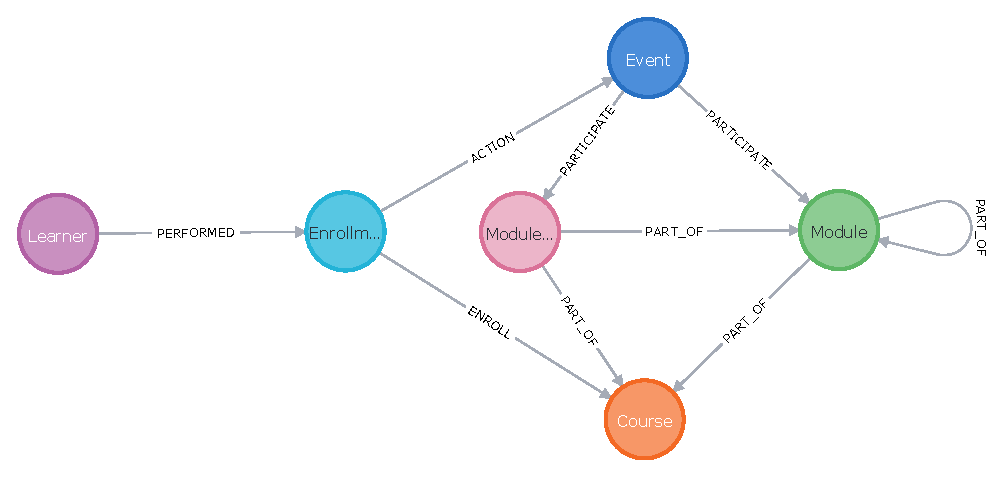
\includegraphics[width=0.45\textwidth]{assets/graph-modeling}
        }
        \caption{แบบจำลองความสัมพันธ์ของกราฟในฐานข้อมูล}
        \label{fig:graph-modeling}
    \end{figure}

    \bibliographystyle{IEEEtran}
    \bibliography{sna-ref}
\end{document}